\documentclass[a4paper,10pt,oneside]{article}
\usepackage[polutonikogreek,italian]{babel}
\usepackage[utf8x]{inputenc}
\usepackage{amsmath}
\usepackage{amsthm}
\usepackage{amssymb}
\usepackage{amscd}
\usepackage{graphicx}
\usepackage{float}
\usepackage{array}
\usepackage{rotating}
\usepackage[small]{caption}
\usepackage{lscape}
\usepackage{fancybox}
\usepackage{booktabs}
\usepackage[noanswer]{exercise}
\parindent0ex
\renewcommand{\fboxsep}{0.4cm}
\usepackage{hyperref}
\renewcommand{\textfraction}{0.05}
\renewcommand{\topfraction}{0.95}
\renewcommand{\bottomfraction}{0.95}
\renewcommand{\floatpagefraction}{0.35}
\renewcommand{\ExerciseName}{Esercizio}
\renewcommand{\ExerciseListName}{Es}
\setcounter{totalnumber}{5}
\restylefloat{figure}
\begin{document}
\section*{Vettori: il prodotto scalare}

\vspace{1cm}

Definiamo come prodotto scalare tra due vettori $\mathbf{U}$ e $\mathbf{V}$ il numero che si ottiene moltiplicando il prodotto dei loro moduli per il coseno dell'angolo tra essi compreso. Il risultato ottenuto è uno scalare, l'operazione appena descritta si indica con un punto:
\begin{equation}
 \mathbf{U}\cdot\mathbf{V}\equiv UV\cos\theta
\end{equation}
dove $\theta$ è l'angolo compreso tra i due vettori leggeremo l'operazione come: $\mathbf{U}$ scalare $\mathbf{V}$. Dalla definizione possiamo notare che il prodotto scalare è commutativo ovvero:
\begin{equation}
 \mathbf{U}\cdot\mathbf{V}=\mathbf{V}\cdot\mathbf{U}
\end{equation}
Se i due vettori formano tra loro un angolo compreso tra $\pi/2$ e $3/2\pi$ il coseno è negativo e di conseguenza il prodotto scalare sarà negativo se $\mathbf{U}=\mathbf{V}$ allora:
\begin{equation}
 \mathbf{V}\cdot\mathbf{U}=U^2=V^2=|\mathbf{U}|^2.
\end{equation}
Se i vettori tra cui eseguiamo il prodotto scalare sono dei versori avremo:
\begin{equation}
 \hat{\mathbf{U}}\cdot \hat{\mathbf{V}}=\cos\theta
\end{equation}
ovvero il prodotto scalare tra due versori coincide con il coseno dell'angolo tra essi compreso.
Notiamo che in virtù della definizione, il prodotto scalare di due vettori può essere nullo senza che lo siano i suoi operandi è sufficiente, infatti, che sia nullo il coseno dell'angolo tra i due. Quindi se $\theta=\pi/2$ o $\theta=3/2\pi$ il prodotto scalare di $\mathbf{U}$ e $\mathbf{V}$ risulta nullo.
Il prodotto scalare risulta estremamente utile nella determinazione delle proiezioni di un vettore sull'altro. Possiamo scrivere la proiezione di $\mathbf{U}$ nella direzione di $\mathbf{V}$ come:
\begin{equation}
 \mathbf{U}\cdot\hat{\mathbf{V}}
\end{equation}
e la proiezione di $\mathbf{V}$ nella direzione di $\mathbf{U}$ come:
\begin{equation}
 \mathbf{V}\cdot\hat{\mathbf{U}}
\end{equation}

\begin{figure}[H]
 \centering
 \includegraphics[width=0.8\textwidth]{./immagini/prodotto_scalare.png}
 % prodotto_scalare.png: 1617x933 pixel, 288dpi, 14.29x8.24 cm, bb=0 0 405 234
 \caption{Il prodotto scalare tra due vettori $\mathbf{U}$ e $\mathbf{V}$ può essere interpretato come $|\mathbf{V}|$ volte la proiezione di $\mathbf{U}$ su $\mathbf{V}$ che come $|\mathbf{U}|$ volte la proiezione di $\mathbf{V}$ su $\mathbf{U}$ }
 \label{fig:prodotto_scalare}
\end{figure}


Notiamo che non esiste l'operazione inversa del prodotto scalare se scriviamo:
\begin{equation}
 \mathbf{U}\cdot\mathbf{X}=z
\end{equation}
il vettore $\mathbf{X}$ \textbf{non} è univocamente determinato a partire da $\mathbf{U}$ e $z$. La divisione tra vettori non è quindi un'operazione definita.


\end{document}
